\section{Phong Reflection Model}

\begin{figure}[H]
  \centering
  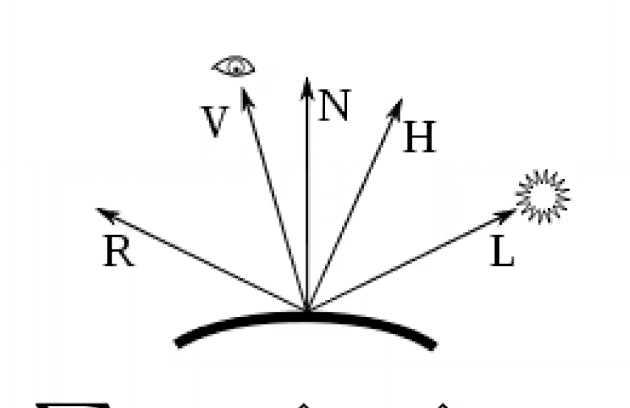
\includegraphics[width=0.7\columnwidth]{images/shading/phong.png}
\end{figure}

\begin{equation}
  I_{p} = k_{a} i_{a} +
  \sum_{m \in \text{lights}}
  \left(
    k_{d} \left( \hat{L}_{m} \cdot \hat{N} \right) i_{m, d} +
    k_{s} \left( \hat{R}_{m} \cdot \hat{V} \right)^{\alpha} i_{m, s}
  \right)
\end{equation}

\begin{itemize}
  \item $ \vec{N} $: normal vector
  \item $ \vec{L} $: direction to light; light has
  \begin{itemize}
    \item Position
    \item Color
  \end{itemize}
  \item $ \vec{V} $: direction to viewer
  \item $ \vec{R} $: reflection vector; mirror reflection direction; light
  vector reflected around the normal
  \begin{equation}
    \vec{R} = 2 \left( L \cdot N \right) N - L
  \end{equation}
  \item $ I_{p} $: the output RGB triple for a vertex
  \item $ k $: material reflectivity; what kind of light reflects from a
  surface; \textbf{material color}
  \begin{itemize}
    \item Each term has its own material color for artistic reasons
  \end{itemize}

  \item $ i_{m} $: $ \left( r, g, b \right) $ for a single light $ m $
  \begin{itemize}
    \item Each term has its own light color for artistic reasons
  \end{itemize}

  \item $ \alpha $: shiniess
  \item All vectors are unit vectors
\end{itemize}

\subsection{Terms}

  \subsubsection{Ambient Term}

    \begin{equation}
      k_{a} i_{a}
    \end{equation}

    \begin{itemize}
      \item $ k_{a}, i_{a} $: $ a $ stands for ambient
      \item Ambient term \textbf{models indirect light}, aka. environment light
    \end{itemize}

  \subsubsection{Diffuse Term}

    \begin{equation}
      k_{d} \left( \hat{L}_{m} \cdot \hat{N} \right) i_{m, d}
    \end{equation}

    \begin{itemize}
      \item $ k_{d}, i_{m, d} $: $ d $ stands for diffuse
      \item $ \hat{L}_{m} \cdot \hat{N} $: the angle between $ L $ and $ N $
      (which are unit vectors)
      \item \textbf{Diffuse reflection is strongest when $ L $ is
      the same as $ N $, i.e. perpendicular to the surface}
      \item Models an idealized\footnote{scatter light uniformly} surface
      (aka, \textbf{rough surfaces})
    \end{itemize}

  \subsubsection{Specular Term}

    \begin{equation}
      k_{s} \left( \hat{R}_{m} \cdot \hat{V} \right)^{\alpha} i_{m, s}
    \end{equation}

    \begin{itemize}
      \item $ k_{s}, i_{m, s} $: $ s $ stands for specular
      \item $ \hat{R}_{m} \cdot \hat{V} $: the angle between reflection and
      the eye
      \item \textbf{Specular reflection is the strongest when the eye aligns
      with the reflection vector}
      \item Specular terms models shiny surfaces
      \item \textbf{Shinier}: a higher $ \alpha $; \textbf{rougher}:
      lower $ \alpha $
      \begin{itemize}
        \item Perfect vs. glossy specular reflection
      \end{itemize}
    \end{itemize}

\subsection{Attenuated Light}

    Add a term in the front of summation; light should decrease as distance
    increases
    \begin{equation*}
      \frac{1}{ad^{2} + bd + c}
    \end{equation*}

    \begin{itemize}
      \item $ d $ is the distance from light to surface
      \item $ a, b, c $ are constants to be adjusted for different effects
    \end{itemize}

\subsection{Open Questions}

  \begin{itemize}
    \item \textbf{When there are no specular surfaces, no moving light}:
    colors of vertices can be optimized to be precomputed at the start and
    be reused later on

    \item \textbf{Modeling 3 wavelength is sufficient} because most people
    have 3 tones in eyes (the three tones are similar to R, G, B)
  \end{itemize}

\subsection{Blinn Phong Model}

  \begin{equation}
    H = \frac{L + V}{\left| L + V \right|}
  \end{equation}

  \begin{itemize}
    \item $ L $: the light
    \item $ V $: the viewer
  \end{itemize}

  In Blinn Phong model, replace $ \left( V \cdot R \right)^{\alpha} $ with
  $ \left( N \cdot H \right)^{b} $

  \begin{itemize}
    \item Slightly cheaper than the Phong model
    \item Only different in specular highlight; not as smooth
    \item Claimed to be more physically correct
    \item Higher $ b > \alpha $ would give an output that is similar to blin
    phong model with $ \alpha $
  \end{itemize}
